\begin{center}
\begin{LARGE}
\title{\textbf{Anna Moroń}}
\end{LARGE}
\end{center}
\section{Sudoku}

\subsection{Troche o pochodzeniu sudoku:}
\begin{flushleft}
\textbf{Sudoku} zostało wynalezione przez Amerykanina Howarda Garnsa w 1979 r. i opublikowane pod nazwą \textit{„Number Place”}. \par

\underline{Łamigłówka przeszła wiele zmian.} Dzisiejsze sudoku pojawiło się po raz pierwszy w Japonii w 1986 r., w czasopiśmie Nikoli, jednak międzynarodową sławę zyskało dopiero w 2005 r.
\end{flushleft} 

\subsection{Wymagane umiejętności:}
\begin{center}
W przeciwieństwie do innych łamigłówek sudoku nie wymaga od gracza wykonywania żadnych rachunków matematycznych, przez co \emph{wydaje się prosta}. W rzeczywistości bez cierpliwości oraz umiejętności logicznego myślenia rozwiązanie diagramu nie jest możliwe.

Do diagramu cyfry wpisywać należy jedynie w miejsca, gdzie cyfra na pewno powinna się znajdować. Niepewne miejsca można tylko zanotować lub zaznaczyć, by uniknąć kreślenia i poprawek.

Poniżej przedstawione są podstawowe metody rozwiązywani
\end{center} 

\subsection{Zasady wypełniania sudoku 9x9:}
\begin{enumerate}
    \item w każde pole wpisuje się jedną cyfre z przedziału 1 do 9
    \item w każdej kolumnie i wierszu powinny znaleść się wszystkie cyfry od 1 do 9, bez powtórzeń
    \item w każdym podkwadracie 3x3 również powinny znaleść się wszystkie cyfry od 1 do 9, bez powtórzeń
    \end{enumerate} 

Dla lepszego wyobrażenia sobie zasad popatrz na przykładową plaszę - tabela \ref{tab:sudokutabela} na stronie \pageref{tab:sudokutabela}.
\begin{table}[htbp]
\centering 
\begin{tabular}{||c|c|c||c|c|c||c|c|c||}
\hline \hline
 & 7 & 8 &  &  &  &  &  & 1 \\ \hline
 &  & 2 & 1 &  &  & 6 &  & 4 \\ \hline
 &  &  & 6 &  &  &  & 8 &  \\ \hline \hline
 & 5 &  &  &  &  &  &  &  \\ \hline
7 &  & 4 & 3 &  &  &  &  & 8 \\ \hline
 &  &  &  &  &  &  & 9 & 7 \\ \hline \hline
3 &  &  & 5 &  &  &  &  &  \\ \hline
 &  &  &  &  &  &  &  & 2 \\ \hline
 & 1 &  &  & 3 & 4 & 5 &  &  \\ \hline \hline
\end{tabular} 
\label{tab:sudokutabela}
\caption{Przykładowa plansza sudoku}
\end{table}


\subsection{Istnieją też inne odmiany sudoku na przykład:}
    \begin{itemize}
        \item[-]sudoku nieregularne, gdzie zamiast 9-polowych kwadratów występują tu 9-polowe figury o nieregularnych kształtach
        \item[-]sudoku diagonalne, gdzie cyfry nie mogą się powtarzać również po przekątnych kwadratu
        \item[-]killer sudoku, gdzie początkowa plansza nie ma żadnych wpisanych cyfr, ale zamiast tego ma zaznaczone obszary obejmujące od 2 do 7 pól, dla których podana jest suma zawartych w nich cyfr (Zobacz zdjęcie \ref{fig:sudokuprzyklad} na stronie \pageref{fig:sudokuprzyklad})
        \item[-]sudoku samurai, składa się z pięciu kwadratów połączonych w kształt litery X 
        \item[-]sudoku trójwymiarow, w kształcie szceściennej kostki 9x9x9 
        \item[-]sudoku magnetyczne, gdzie niedozwolone jest stykanie się tych samych cyfr na rogach kwadratów
    \end{itemize}

\begin{figure}[htbp]
    \centering
    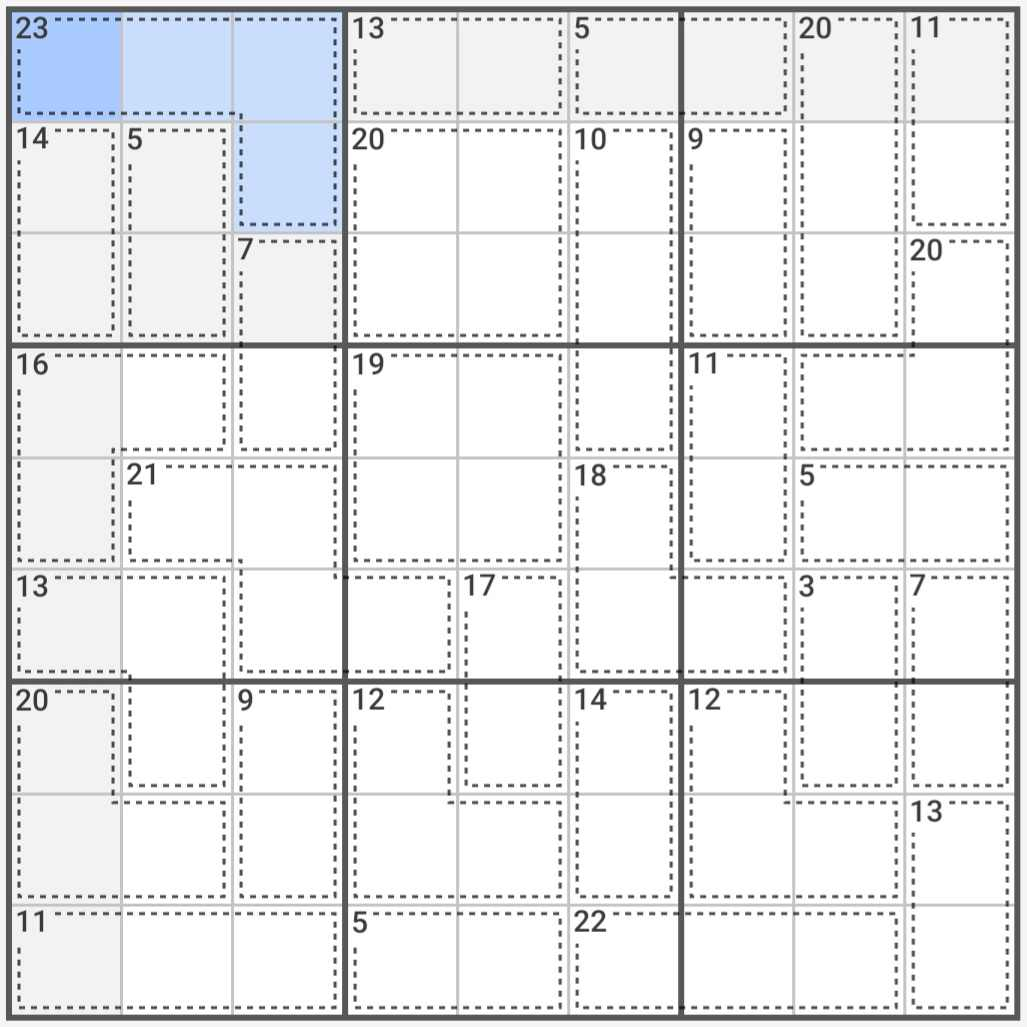
\includegraphics[width=0.75\textwidth]{pictures/sudokuprzyklad.jpg}
    \caption{Przykładowy wygląd planszy killer sudoku}
    \label{fig:sudokuprzyklad}
\end{figure} 

\subsection{Tu przydało by sie wyrażenie matematyczne:}
Dobrymi przykładami będą wzory podstawowowe całek nieoznaczonych. \\Pierwszy przykład: \( \int \frac{1}{sin^2 x}dx = -ctg x +c \) i drugi: 
\begin{equation}
    \int \frac{1}{\sqrt{1-x^2}}dx = arcsin x+c
\end{equation}
